\documentclass[
	12pt
] {article}

\usepackage[
	a4paper,
	left=3cm,
	right=2cm,
	top=3cm,
	bottom=3cm
] {geometry} %for setting margin

\usepackage{parskip}
\usepackage{mathtools}
\usepackage{authblk} %authors and their affiliations
\usepackage{graphicx} %for include graphics
\graphicspath{{figures/}}

\title{Two-phase imbibition in Porous Media using a Two-dimensional Network Model}

\author[1, 2]{Kafi Shabbir}
\author[1, 3]{Oleg Izvekov}
\author[1, 4]{Andrey Konyukhov}
\affil[1]{Moscow Institute of Physics and Technology, Dolgoprudny, 141701}
\affil[2]{kafiulshabbir@phystech.edu}
\affil[3]{izvekov\_o@inbox.ru}
\affil[4]{konyukhov\_av@mail.ru}

\begin{document}
\nocite{*}
\maketitle
UDK: 532.685

\begin{abstract}
	 This article is about a 2D network model, which we developed for simulating imbibition of two-phase flow in porous media. Our 2D plane of porous media consisted of two regions: the outer region with thicker tubes was initially saturated with wetting fluid, and the inner region with thinner tubes with non-wetting fluid. We measured the saturation of wetting fluid $S$  with respect to time $t$, and the average capillary pressure $P_c$ with respect to $S$ in the inner region. Our network model used a novel method of distributing fluids at the nodes, which is when more than two phases enter a node at the same time, the wetting fluid is distributed first according to the ascending order of the radii of the tubes. Simulation results showed that the wetting fluid indeed invaded the inner region and displaced the non-wetting fluid to the outer region, and the plots of $S(t)$ and $P_c(S)$ qualitatively matches other references. Therefore, the novel method of distributing different phases at nodes and our network model is valid in general.
\end{abstract}

\textbf{Keywords:} imbibition, capillary pressure, non-equilibrium effect, phase distribution

This project was supported by Russian Science Foundation, grant 23-21-00175.

\section{Introduction} \label{sec:intro}
	Modeling and simulation of two-phase flow in porous media is important due many applications in oil recovery, hydrology, electricity production, etc \cite{labed2012experimental}. Porous media consists of a skeletal material (usually solid) and voids (also called pores). The voids are connected to each other by other narrow tube like voids called capillaries. The voids are usually filled with fluids such as water, oil or gases \cite{su2012insights}. Saturation of a fluid $S_i$ is defined as the ratio between the volume $V_{i}$ occupied by ${fluid}_i$ to the total volume of the void $V_{void}$:
	
	\begin{equation}
		S_{i} = \frac{V_{i}}{V_{void}}
	\end{equation}
	
	Since we consider only two fluids: wetting of saturation $S_w$ such as water, and non wetting of saturation $S_{nw}$ such as oil in the voids. The two quantities are related such that: $S_{w} + S_{nw} = 1$. For simplicity, let $S$ denote the saturation of the wetting fluid. Classical continuum models, such as Darcy's Law \cite{darcy1856fontaines} are still commonly used:
	\begin{equation}
		q = -\frac{k}{\mu} \nabla P
	\end{equation}
	
	Here, $q$ is the flow rate, $k$ is the permeability, $\mu$ is the coefficient of viscosity, and $\nabla P$ is the pressure gradient.
	
	In classical continuum models, the permeability is only a function of the saturation of one of the fluid $k = k(S)$ \cite{kondaurov2007thermodynamically} \cite{kondaurov2009non}.
	
	The classical continuum models are valid as long as the characteristic time of the processes is much longer than the characteristic time of fluid redistribution in the capillary space. The fluid distribution can take longer time due to non-equilibrium effects, which occurs when the saturation changes rapidly, or the porous medium is fractured with blocks and cracks \cite{barenblatt1960basic} \cite{barenblatt2003mathematical}. In these cases, the assumption that permeability is only a function of the saturation is not sufficient, and additional parameters are required. Various advanced continuum models \cite{hassanizadeh2004continuum}, \cite{hassanizadeh1987high}, \cite{barenblatt1960basic} consider such non-equilibrium effects, by assuming the permeability $k$ to additionally be a function of the rate of change of saturation with respect to time:
	
	\begin{equation} \label{eq:conn-adv-model-perm}
		k = k(S, \frac{\partial S}{\partial t})
	\end{equation}

	Nevertheless, the process of redistribution of fluids in the pore space can occur even at constant saturation $S = const$, to take this into account, Kondaurov proposed including an additional special non-equilibrium parameter  $\xi$, which relaxes to an equilibrium value \cite{kondaurov2007thermodynamically} \cite{kondaurov2009non}:
	
	\begin{equation}
		k = k(S, \xi)
	\end{equation}
	
	And $\xi$ is related to $S$ by a differential equation:
	
	\begin{equation}
		\frac{\partial \xi}{\partial t} = \Omega ( S, \xi )
	\end{equation}
		
	Here, $\Omega$ is a function [COMMENT: verification needed].
	
	In order to better understand the non-equilibrium characteristics, it is necessary to develop non-continuum models and simulate the flow at the scale of pores. Some of the methods of modeling at the scale of pores are: Lattice Boltzmann Method \cite{chen1998lattice}, a direct Navier-Stokes simulation, or a network model [REF? Need help to find proper Citation about article which speaks about the various methods used to model non-continuum characteristics of porous media]. Direct Navier-Stokes simulation gives us very accurate results on velocity and pressure distributions, but it is very complicated [REF?, add citation]. Network models are much simpler. We have developed a network model and simulated a particular phenomena, imbibition, to understand the non-equilibrium characteristics of two-phase flow, and observe the Kondaurov's non-equilibrium parameter resting at an equilibrium value.
	
\section{Theory}
\subsection{Characteristics of our network model}
	\begin{figure}
		\centering
		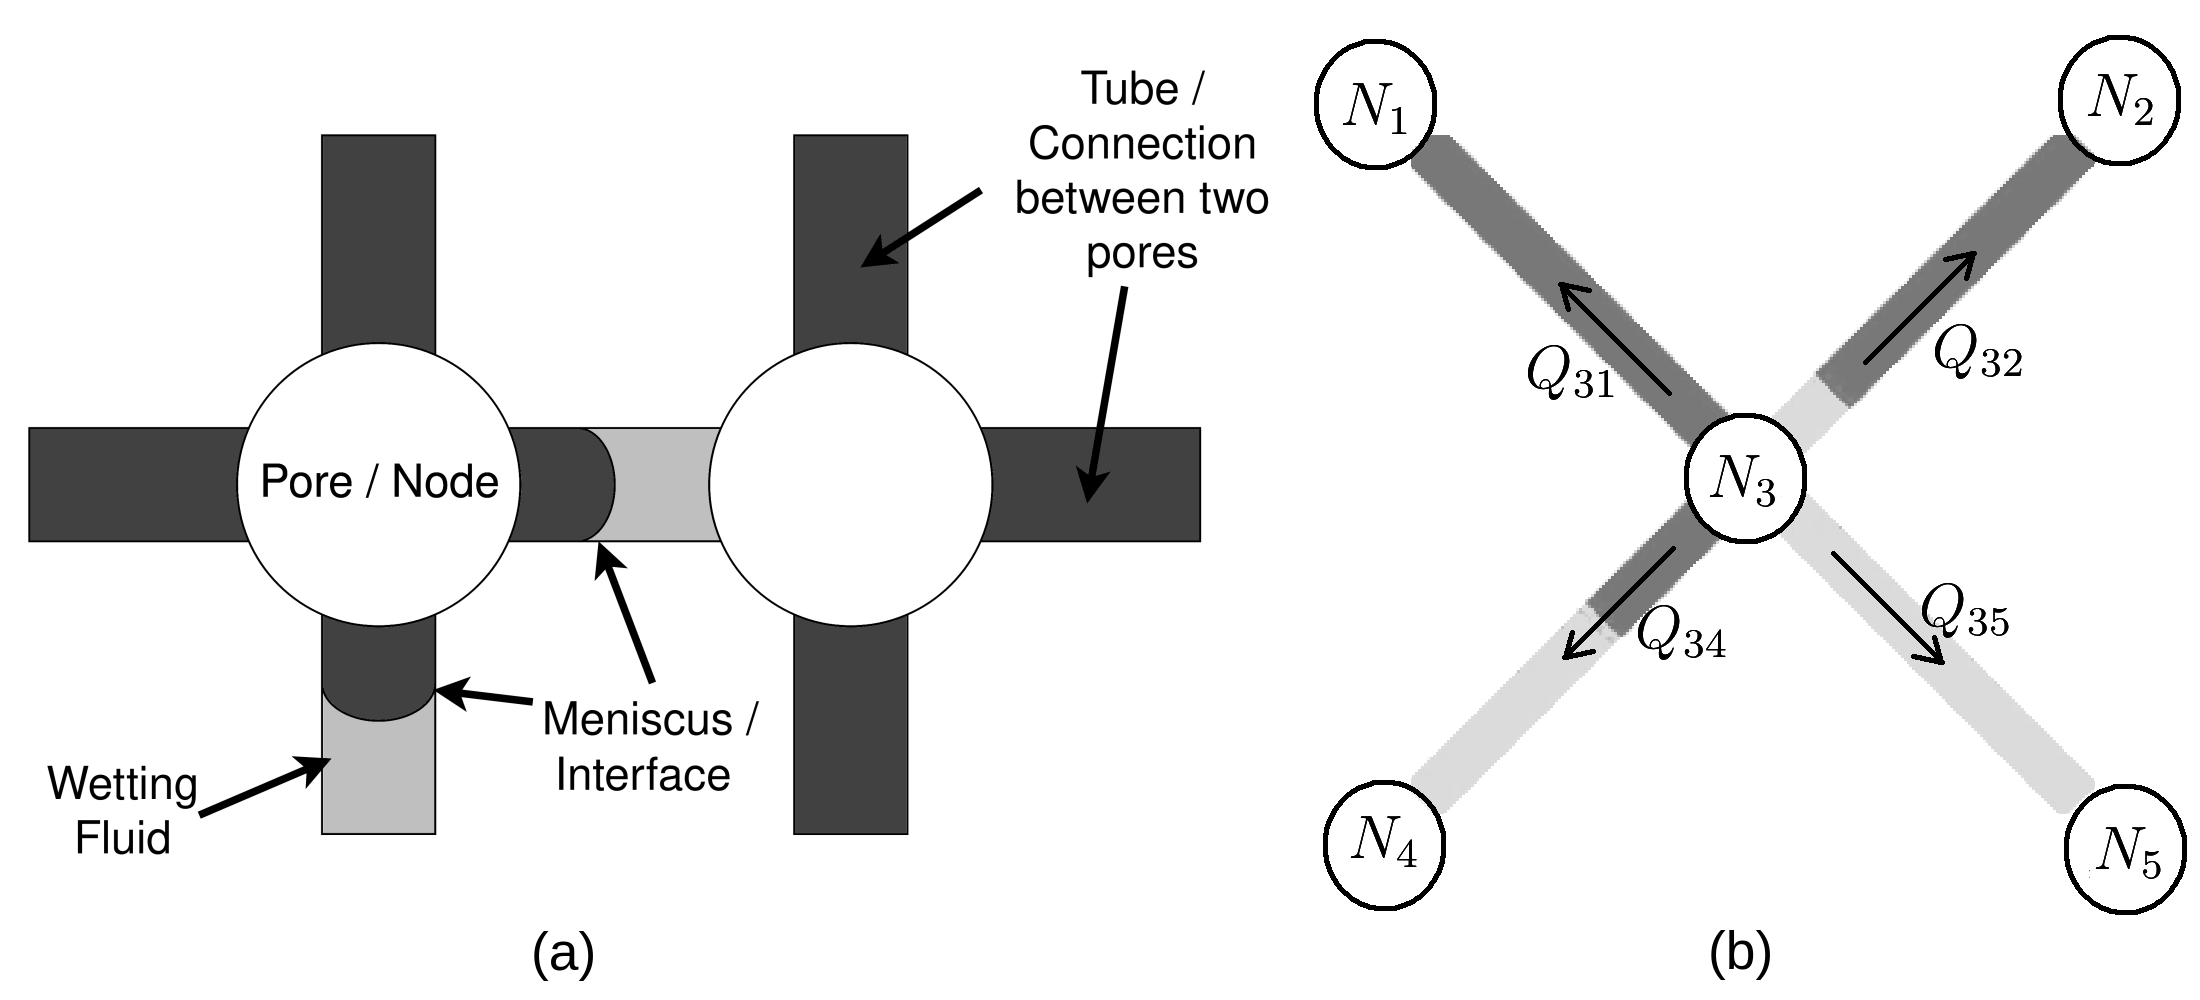
\includegraphics[width=\textwidth]{fig_1_2200x1000}
		\caption{Network model as an approximation of porous media (a), with pores as nodes, and capillaries as tubes. Flow rates $Q$ out of Node $N_3$ (b).}
		\label{fig:1}
	\end{figure}
	
	In our network model, the pores are represented by nodes, and capillaries by tubes, as shown in figure \ref{fig:1}a. Our model is two-dimensional (2D), and each node is connected to 4 other nodes by tubes of the same length, as also shown in figure \ref{fig:1}b. In our model, the tubes can have different radii, and a maximum of 2 menisci. The flow is always viscous and laminar. A node may be connected to less than 4 nodes, when they are located at the boundaries, see figure \ref{fig:3}. The fluids are not compressible. The darker color always denotes non-wetting fluid, while the lighter color denotes wetting fluid. Gravity is ignored. The volume of the node is not taken into consideration and is assumed to be zero.
	
	Our model has some similar features as \cite{aker1998two}. However, they considered tubes to be hour glass shaped and used approximate flow rate equations \cite{washburn1921dynamics}, while we used only cylindrical tubes, because it allowed us to derive and use exact flow rate equations. \cite{aker1998two} had to consider the nodes to have volume, which complicates the determination of saturation in a region, while we have assumed the nodes to have zero volume since assigning volume would not affect the characteristic of our flow.
	
	\begin{figure}
		\centering
		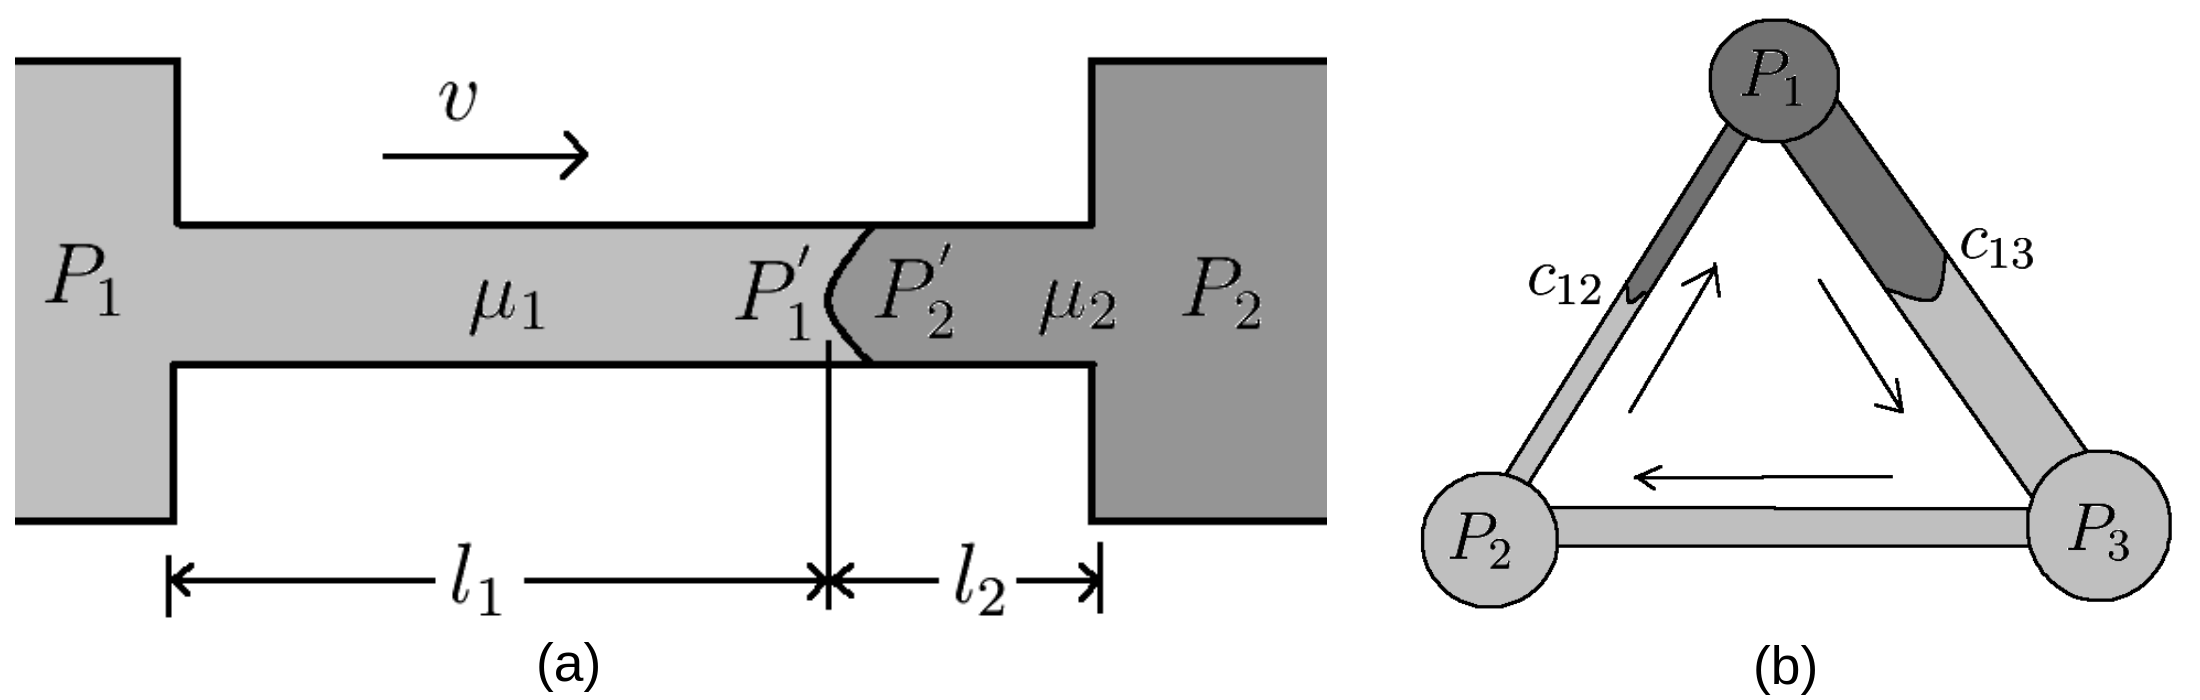
\includegraphics[width=\textwidth]{fig_2_2200x700}
		\caption{Flow in a tube with a meniscus and fluids of viscosity $\mu$,  (a). A simple example of a system with menisci and closed boundaries (b), where the pressure matrix has infinitely many solutions.}
		\label{fig:2}
	\end{figure}
	
\subsection{Average capillary pressure}
	The capillary pressure $p'$ is:
	\begin{equation} \label{eq:surface-tension}
		p' = \frac{2 \sigma}{R}
	\end{equation}
	
	Here, $\sigma$ is the coefficient of surface tension in $[Pa.m]$ or $[kg/s]$, $R$ is the radius of the tube.
	
	Let us define an function $Z$ dependent on the number of meniscus $n_{mns}$:
	\begin{equation} \label{eq:average-capillary-pressure-sign}
		Z(n_{mns}) = 
		\begin{dcases}
			0,&\text{$n_{mns}$ = 0, 2}\\
			1,&\text{$n_{mns}$ = 1}\\
		\end{dcases}
	\end{equation}
	
	We define the average capillary pressure $P_c$ in a region as:
	\begin{equation} \label{eq:average-capillary-pressure}
		P_c = \frac{\sum p'_i Z_i \pi R_i^2}{\sum Z_i \pi R_i^2}
	\end{equation}
	
\subsection{Flow rate in a tube with meniscus}
	The pressure jump across a meniscus for the tube in figure \ref{fig:2}a:
	\begin{equation} \label{eq:pressure-jump-def} 
		 p' = P_{2}' - P_{1}'
	\end{equation}
	
	Here, $p'$ is from equation \ref{eq:surface-tension}.
	We define the average viscosity parameter $M$, for a tube with multiple fluids of different viscosity $\mu$:
	\begin{equation} \label{eq:def-average-viscosity}
		M = \sum_{i} \mu_{i} \frac{l_{i}}{l}
	\end{equation}
	
	Here, $\mu$ is the dynamic viscosity in $[kg/m.s]$, $l$ is the length of the tube.
	
	In figure \ref{fig:2}a, for simplicity let $P_1 > P_2$ and the convex side of the meniscus be pointing towards the node $N_1$ which is at pressure $P_1$. Then the velocity will be from node $N_1$ to node $N_2$, since both the pressure difference ($P_1 > P_2$) in the nodes and the capillary pressure produces a force to move the fluid from $N_1$ to $N_2$. We can perform the following steps:
	\begin{enumerate}
		\item Write Hagen–Poiseuille equation \cite{sutera1993history} for parts of tubes of with same viscosity separately. For example, in figure \ref{fig:2}a: $Q(\mu_1 l_1) = A' (P_1 - P'_1)$ and $Q(\mu_2 l_2) = A' (P'_2 - P_2)$, here $A' = \pi R^4 / 8$
		\item Sum the Hagen–Poiseuille equations.
		\item Replace the pressure jump $P'_2 - P'_1$ according to equation \ref{eq:pressure-jump-def}, and average viscosity parameter $M$ according to equation \ref{eq:def-average-viscosity}.
	\end{enumerate}
	And the flow rate for a tube with a pressure difference in the nodes and a meniscus:
	\begin{equation} \label{eq:flow-rate-main}
		Q = \frac{\pi R^4}{8Ml} \left( \Delta P_{12} + \frac{2 \sigma}{R} \right)
	\end{equation}
	
	Here, $Q$ is the volumetric flow rate in $[m^3/s]$, and $\Delta P_{12} = P_1 - P_2$.
	
	Let us consider flow from an arbitrary Node $N_i$ to Node $N_j$, and $X_{ij}$ is any quantity $X$ associated with the tube connecting $N_i$ and $N_j$. We define $s$ to be a function which can only take the values of: $-1, 0, +1$, according to the orientation and the number of menisci present in the tube:
	
	\begin{equation}
		s_{ij}(d, n_{mns}) = 
		\begin{dcases}
			-1,&\text{$n_{mns}$ = 1, $d$ points away from $N_{i}$}\\
			0,&\text{$n_{mns}$ = 0, 2}\\
			+1,&\text{$n_{mns}$ = 1, $d$ points towards $N_{i}$}
		\end{dcases}
	\end{equation}

	Here, $d$ is the direction the convex side of the meniscus points towards. $n_{mns}$ is the number of meniscus in a tube.
	
	The flow rate equation of any $n_{mns}$ is:
	
	\begin{equation} \label{eq:flow-rate-simple}
		Q_{ij} = A_{ij}\Delta P_{ij} + B_{ij}
	\end{equation}
	
	Here, $\Delta P_{ij} = P_i - P_j$, and:
	\begin{equation} \label{eq:flow-rate-aij}
		A_{ij} = \frac{\pi R_{ij}^4}{8M_{ij}l}
	\end{equation}
	
	\begin{equation} \label{eq:flow-rate-bij}
		B_{ij} = \frac{\pi R_{ij}^4}{8M_{ij}l} \frac{2 s_{ij} \sigma}{R_{ij}}
	\end{equation}
	
	
	Since $M_{ij} = M_{ji}$ and $s_{ij} = -s_{ji}$, we obtain:
	\begin{equation} \label{eq:symm-a-ij}
		A_{ij} = A_{ji}
	\end{equation}
	\begin{equation} \label{eq:symm-b-ij}
		B_{ij} = -B_{ji} 
	\end{equation}
	
	The flow velocity is:
	\begin{equation} \label{eq:vel-from-flow-rate}
		v_{ij} = \frac{ Q_{ij} }{\pi R_{ij}^2}
	\end{equation}
	
\subsection{Open system: filtration}
	In an open system, we can externally supply or remove fluid from the set of nodes and tubes. Filtration is an example open system. For example, we have a block of porous media saturated with water. On the front face we apply high pressure of air, and keep the back face at a lower pressure. The air invades the porous block from the front face, and the water leaves the porous block from the back face. 
	
	Figure \ref{fig:1}b is a very simple case of filtration. Here $N_4$ and $N_5$ are open and maintained at a constant higher pressure, while $N_1$ and $N_2$ are maintained at a constant lower pressure. We need to calculate the velocity at which the menisci will displace in each tube. The steps are:
	
	\begin{enumerate}
		\item Assume the pressures to be the variables for the nodes where the pressure is not known.
		
		\item Write the of set linear equations using equation \ref{eq:flow-rate-simple}.
		
		\item Solve the set of linear equations to determine pressures in all nodes.
		
		\item Use equation \ref{eq:flow-rate-simple} again to determine the flow rates in each tube.
		
		\item Find velocity at which the menisci will displace using equation \ref{eq:vel-from-flow-rate}.
	\end{enumerate}
		
	Let us apply the steps to figure \ref{fig:1}b. Here, the pressure is not known only in $N_3$. Since the fluids are not compressible, the sum of volumetric flow out of $N_3$ is zero, or Kirchhoff's law is satisfied in $N_3$:
	
	\begin{equation} \label{eq:sum-flow-node-zero}
		\sum_{k} Q_{3k} = 0
	\end{equation}

	Here, $k = (1, 2, 4, 5)$. If we have two linear equations $a_1 P_1 + b_1 P_2 = c_1$ and $a_2 P_1 + b_2 P_2 = c_2$, if $P_1$ and $P_2$ are the variables here, then the augmented matrix for pressure (pressure matrix) is:
	
	\begin{equation}
		\begin{pmatrix}
			a_1 & b_1 & c_1\\
			a_2 & b_2 & c_2
		\end{pmatrix}
	\end{equation}
	
	For figure \ref{fig:1}b, the pressure matrix is:
	
	\begin{equation} \label{eq:matrix-open-sys-5-nodes}
		\begin{pmatrix}
			1 & 0 & 0 & 0 & 0 & P_{1}\\
			0 & 1 & 0 & 0 & 0 & P_{2}\\
			-A_{31} & -A_{32} & (A_{31} + ... + A_{35}) & -A_{34} & -A_{35} & -(B_{31} + ... + B_{35})\\
			0 & 0 & 0 & 1 & 0 & P_{4}\\
			0 & 0 & 0 & 0 & 1 & P_{5}
		\end{pmatrix}
	\end{equation}
	
	After solving matrix \ref{eq:matrix-open-sys-5-nodes}, we obtain the pressure at $N_3$, which means we now know the pressures at all nodes, this allows us to find the velocities in each tube.
	
\subsection{Closed system}	
	It can be proven that, we can take a network model of an arbitrary large size, and if we maintain high pressure at the bottom row of nodes, and low pressure on top row, the linear equations produce an unique solution and it is possible to determine the flow rates in all tubes. We have simulated the process of filtration and verified that our model works. However, in order to simulate imbibition, we need a closed system. Figure \ref{fig:2}b is a simple example of a closed system, whose pressure matrix is:
	
	\begin{equation}
		\begin{pmatrix}
			(A_{12} + A_{13}) & -A_{12} & -A_{13} & -B_{12} - B_{13} \\
			-A_{21} & (A_{21} + A_{23}) & -A_{23} & -B_{21} - B_{23} \\
			-A_{31} & -A_{32} & (A_{31} + A_{32}) & -B_{31} - B_{32} \\
		\end{pmatrix}
	\end{equation}
	
	From equation \ref{eq:symm-a-ij} and \ref{eq:symm-b-ij}, we have $A_{ij} = -A_{ij}$ and $B_{ij} = - B_{ji}$, we see that the sum of each column in this matrix is zero. Therefore, there are infinitely many solutions. We have solved this problem by, adding a non zero real constant $a$ to the 3rd column.
	
	\begin{equation}
		\begin{pmatrix}
			(A_{12} + A_{13}) & -A_{12} & -A_{13} + a & -B_{12} - B_{13} \\
			-A_{21} & (A_{21} + A_{23}) & -A_{23} + a & -B_{21} - B_{23} \\
			-A_{31} & -A_{32} & (A_{31} + A_{32}) + a & -B_{31} - B_{32} \\
		\end{pmatrix}
	\end{equation}
	
	Then the sum of all columns give us $3aP_3 = 0$, which means $P_3 = 0$. It can be shown that any node in the system can be assumed to have zero pressure, the pressure difference which determines the flow rate is not affected by the choice of node where we assume zero pressure. Which means in a closed system, we must choose an arbitrary node to have $0$ pressure.

\subsection{Fluid distribution in nodes (novel method)} \label{sec:fluid-distb-exmpl}
	There are situations when both wetting and non-wetting fluid enters a node. According to our novel method, we insert the wetting fluid first into tubes in ascending order of their radius.
	
	For example, let's say that we have solved the set of linear equations and chosen an appropriate time step to integrate, we know the volume of each fluid that will enter the node and will leave the node, their sum must be equal due to the conservation of volume. ${tube}_3$ is thinner than ${tube}_4$. Now let us look at certain cases:
	\begin{enumerate}
		\item $V_{in, w} = 0.6 u$ (unit volumes) of wetting fluid, and $V_{in, nw} = 0.4 u$ of non-wetting fluid enters a node from ${tube}_1$ and ${tube}_2$, it does not matter how much of which fluid came from which tube. And from calculated flow rates, we know that $V_{3} = 0.2 u$ will flow into ${tube}_3$ and $V_4 = 0.8 u$ into $tube_4$:
		
		\begin{enumerate}
			\item Since $V_3 < V_{in, w}$, $V_3 = 0.2 u$ of wetting fluid in inserted into ${tube}_3$.
			\item $V_{4, w} = V_{in, w} - V_3$ which is $0.6 - 0.2 = 0.4 u$ of wetting fluid is first inserted into ${tube}_4$.
			\item Then $V_4 - V_{4, w} = 0.4 u$ of non-wetting fluid is inserted into ${tube}_4$.
		\end{enumerate}
		
		\item $V_{in, w} = 0.3 u$ of wetting fluid, and $V_{in, nw} = 0.7 u$ of non-wetting fluid enters a node from ${tube}_1$ and ${tube}_2$. And from calculated flow rates, we know that $V_3 = 0.5 u$ will flow into ${tube}_3$ and $V_4 = 0.5 u$ into $tube_4$:
		
		\begin{enumerate}
			\item Since $V_3 > V_{in, w}$, $V_{in, w} = 0.3 u$ of wetting fluid in inserted into ${tube}_3$.
			\item Then $V_3 - V_{in, w} = 0.2 u$ of non-wetting fluid is inserted into ${tube}_3$.
			\item ${tube}_4$ is filled with $V_4 = 0.5 u$ of non-wetting fluid.
		\end{enumerate}
	\end{enumerate}


\section{Experiment} \label{sec:rad-distb}
	\begin{figure}
		\centering
		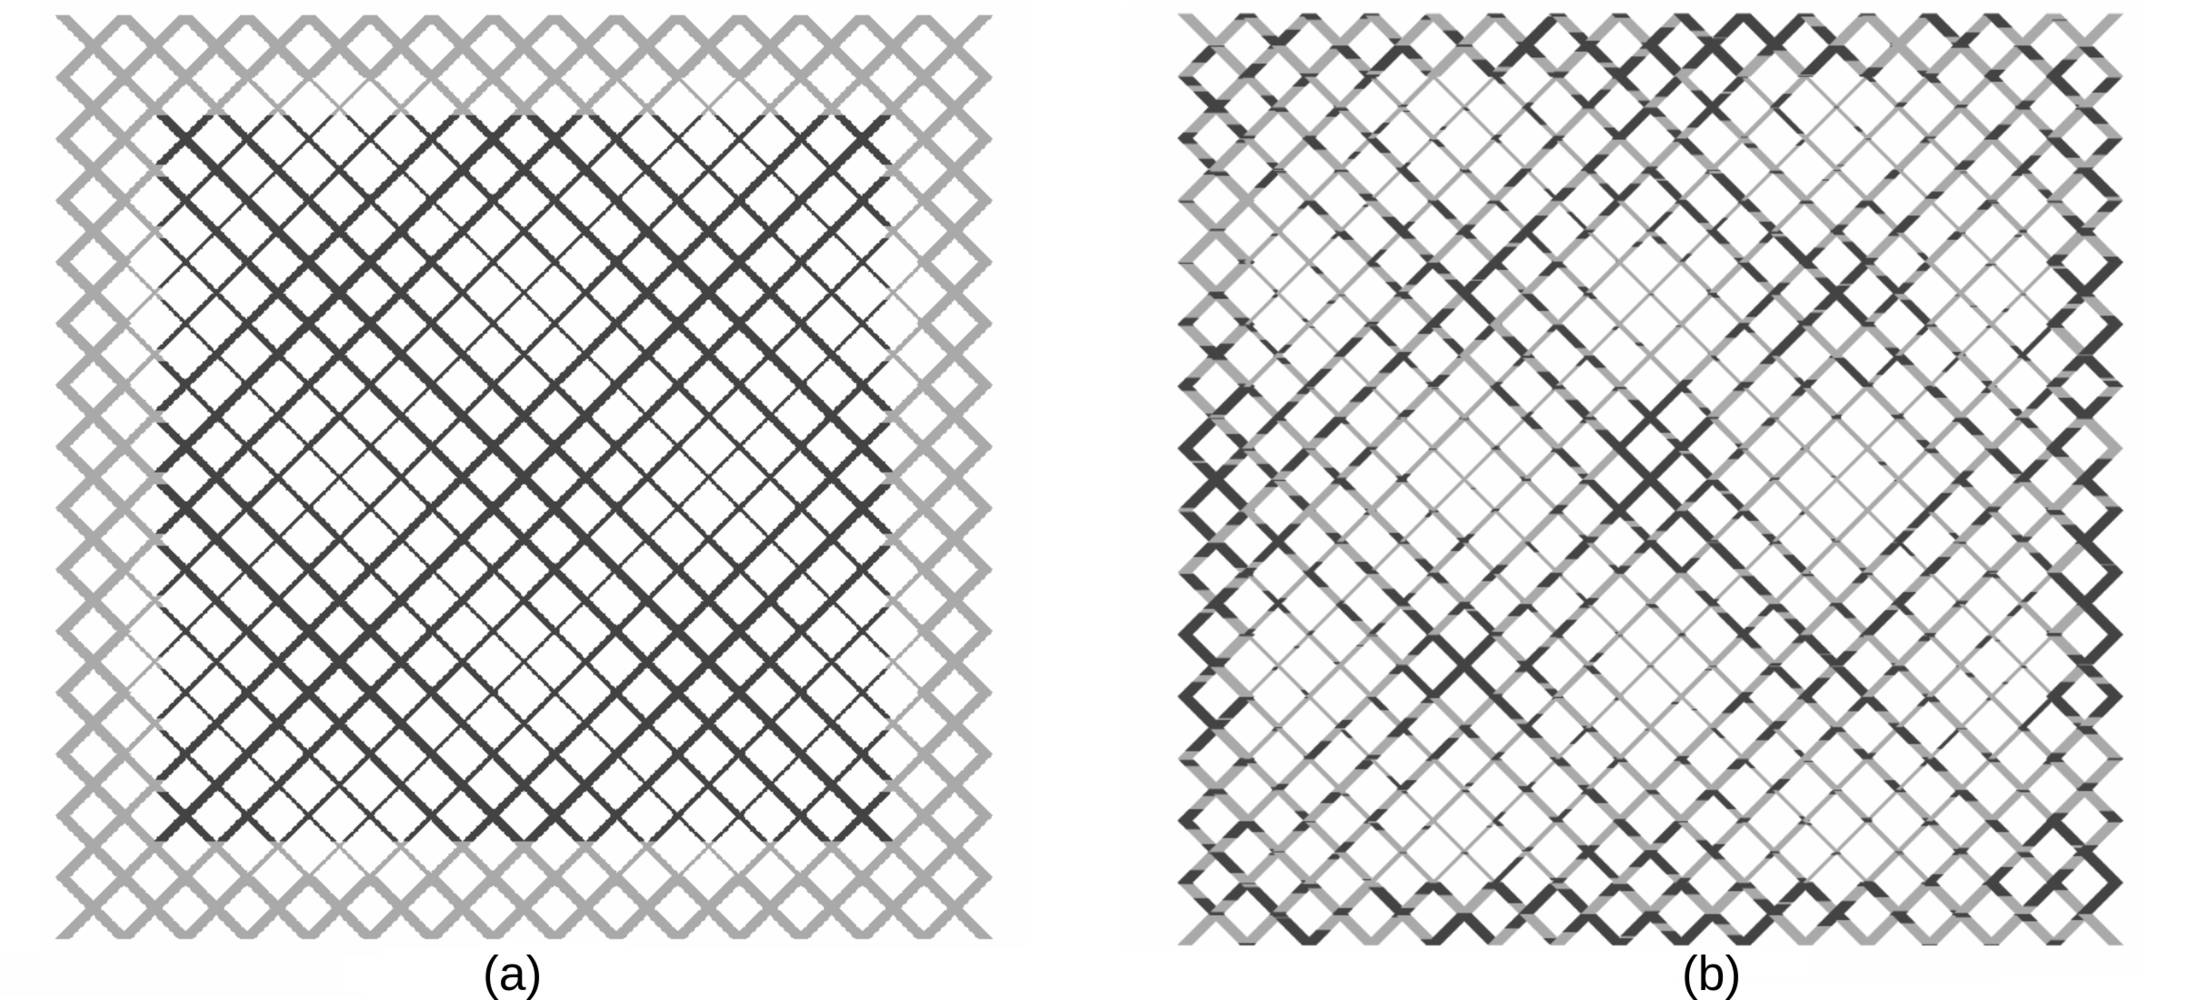
\includegraphics[width=\textwidth]{fig_3_2200x1000}
		\caption{Wetting fluid (lighter color) initially situated in the outer region with thicker tubes, non-wetting fluid (darker color) in the inner region saturated with thicker tubes (a). After simulation and we see that non-wetting fluid (dark) mostly occupies the intersection of the thicker tubes, and wetting fluid (b) occupies the thinner tubes.}
		\label{fig:3}
	\end{figure}

	In the simulation of imbibition, wetting fluid was situated in the outer region, and non-wetting fluid in the inner region as shown in figure \ref{fig:3}a. The capillary pressure at the corners is greater than in the edges. Therefore the wetting fluid invades into the inner region from the corners of the inner region and displaces the non-wetting fluid from the edges. We measure the saturation of wetting fluid $S(t)$ with respect to time in the inner region. And, the final average capillary pressure $P_c$ in the inner region for various different final saturation $S$, then compare the $P_c(S)$ curve obtained to classical literature.
	
	The two rows along the perimeter are set to have the thickest radius of $6 m$, and declared to be the outer region. The inner region constitutes of thinner tubes of radii of range $(2, 3, ..., 5) m$. The volume of the inner region is approximately equal to the volume of the outer region. The main diagonals are the thickest ($5 m$), while the others are thinner by steps of $1 m$. The proportion of volume occupied by tubes in the inner region for various radii is plotted in figure \ref{fig:4}a. Due to the nature of equation \ref{eq:flow-rate-simple} multiplying all radii $R_i$ by a positive real constant only changes the scale of the axes. Since we are interested only in the qualitative shape of the plots, it is not a issue that the capillaries in our simulation are much thicker than in nature. In order to be able to compare the curves of experiments of different radius distributions, we have used dimensionless time in all $S(t)$ plots. 
	
	We perform various experiments with the the same radius distribution, but different initial positions of the menisci in each experiment to change the final saturation. We obtain a $S(t)$ plot for every experiment. And each experiment gives us one point for the $P_c(S)$ plot. 

	
\section{Algorithm}
It is necessary to perform the following steps once before the series of experiments, we have performed 10 such experiments, with final saturation of wetting fluid in inner region ranging from $0.02$ to $0.75$.

\begin{enumerate}
	\item \textbf{Generate radius-distribution-table} of tubes of $30 \times 30$ rows and columns, shown in figure \ref{fig:3} and described in section \ref{sec:rad-distb}.
	
	\item \textbf{Add random} values to each $R$ in the radius-distribution-table. So that, there is always an unique way to distribute different fluids when wetting and non-wetting will flow into a node at the same time (section \ref{sec:fluid-distb-exmpl}). In this experiment $\Delta R/R \approx 10^{-3}$.
	
	\item \textbf{Declare constants} such as ${\mu}_{1}$, ${\mu}_{2}$, $l$, $\sigma$. We show results for ${\mu}_1 = {\mu}_2$, $\sigma = 1 Pa.m$ and $l = 1 m$, we chose simple values so that it will be easy to repeat our results with different models, and we have verified by simulations that the size of these constants only scale the axes and does not affect the general shape of the plots.
\end{enumerate}

The following steps are performed for each experiment.

\begin{enumerate}
	\item \textbf{Generate new meniscus-configuration} such that the convex side of all menisci faced outwards, see figure \ref{fig:3}. We vary the distance of the meniscus from the outside boundary to change the initial saturation of wetting fluid. We have observed that the final saturation of the wetting fluid in the inner region is proportional to the initial saturation of wetting fluid in the system.
	
	\item \textbf{Declare empty pressure-matrix} $M_{ij}$ by filling its $n$ rows and $n + 1$ columns with $0$'s. Here $n$ is the number of nodes in our system.
	
	\item \textbf{Declare time counter} and set the physical time of our simulation $t = 0$.
	
	\item \textbf{Main loop:} run for 10,000 steps or until there is no tube with an odd number of meniscus to continue the flow:
	\begin{enumerate}
		\item \textbf{Generate linear equations} by iterating through every Node $N_i$, $1 \le i \le n$:
		
		\begin{enumerate}
			\item \textbf{Generate connections}, which is the list of nodes $N_j$ and tubes $b_{ij}$, which are connected to $N_i$.
			
			\item \textbf{Sum the flow rates} for each connection, that is for each node $N_j$ connected to $N_i$ by tube $b_{ij}$, a sample of which was described in equation \ref{eq:sum-flow-node-zero}:
			
			\begin{enumerate}
				\item Obtain $R_{ij}$ from the radius-distribution-table.
				
				\item Calculate $M_{ij}$ and $s_{ij}$ from current meniscus configuration of tube $b_{ij}$.
				
				\item Calculate $A_{ij}$ and $B_{ij}$ from $R_{ij}$, $M_{ij}$, $s_{ij}$, and other constants, according to equations \ref{eq:flow-rate-aij} and \ref{eq:flow-rate-bij}.
				
				\item Perform the following modifications to $M_{ij}$:
				
					$M_{ii} = M_{ii} + A_{ii}$
				
					$M_{ij} = M_{ij} - A_{ij}$
				
					$M_{i,n + 1} = M_{i,n + 1} - B_{ij}$
			\end{enumerate}
		\end{enumerate}
		
		\item \textbf{Calculate pressures} in each node by solving the matrix $M_{ij}$. Gaussian-elimination was used for the results of simulations shown in this article. 
		
		\item \textbf{Calculate flow rates} from the pressures calculated in each node using equation \ref{eq:flow-rate-simple}.
		
		\item \textbf{Calculate velocity} from the flow rates using equation \ref{eq:vel-from-flow-rate}.
		
		\item \textbf{Choose a time step} $\Delta t$ for integration. For all tubes $b_{ij}$, calculate $\Delta t_{ij} = \tau l/v_{ij}$. We used $\tau = 0.1$ for all of out simulations. Then $\Delta t = min(t_{ij})$. 
		
		\item \textbf{Declare empty volume-displacement-table} $L$ of $n$ rows and 2 columns, to store the amount of wetting and non-wetting fluid entering any Node $N_i$.
		
		\item \textbf{Populate volume-displacement-table} by iterating through all tubes $b_{ij}$:
		\begin{enumerate}
			\item \textbf{Determine out-flow Node} $N_k$ which receives fluid(s) from tube $b_{ij}$, here $k = i or j$, depending on the direction of velocity in the tube. .
			
			\item \textbf{Find total volume of fluid} $V$ entering $N_k$ from $b_{ij}$, here $V = v_{ij} \Delta t \pi R_{ij}^2$.
			
			\item \textbf{Find volumes of fluids} $V_{w}$ and $V_{nw}$, depending on the presence and position of menisci within the volume which will be removed from the tube in this step, here $V_{w} + V_{nw} = V$.
			
			\item \textbf{Modify the volume-displacement-table:} $L_k(w) = L_k(w) + V_w$ and $L_k(nw) = L_k(nw) + V_nw$
		\end{enumerate}
		
		\item \textbf{Integration} on time to displace the menisci, iterate through all the nodes $N_i$: 
		
		\begin{enumerate}
			\item \textbf{The novel method} for distributing wetting and non-wetting fluid at the nodes, as described in section \ref{sec:fluid-distb-exmpl}:
			\begin{enumerate}
				\item \textbf{List outflow tubes} $b_k$ which take fluids from $N_i$.
				
				\item \textbf{Sort outflow tubes} according to the ascending order of their radii.
				
				\item \textbf{Distribute} the wetting fluids first into the outflow-tubes sorted in the ascending order of their radii, then non-wetting fluid.. 
			\end{enumerate}
			
			\item \textbf{Recombine} when a tube has more than 2 menisci, combine fluids of same viscosity in a tube such that a tube always has 2 or less menisci and the center of mass of the fluids remain the same.
		\end{enumerate}
		
		\textbf{Save results} for every $200$ steps. Because, we wanted our $S(t)$ plots to be have $50$ ($10,000/200$) points. 
		
		\begin{enumerate}
			\item \textbf{Calculate saturation} $S$ of wetting fluid inner region, add this to the plot of $S(t)$, we obtained such $S(t)$ plots for each of the 10 experiments, one of them is figure \ref{fig:4}b.
			\item \textbf{Visualization} of positions of wetting and non-wetting fluids in the tubes. We show the final position of wetting and non-wetting fluid in figure \ref{fig:3}b.
		\end{enumerate}
		
		\item \textbf{Update time:} $t = t + \Delta t$.
	\end{enumerate}
	\item \textbf{Generate video} file for better visualization of the experiment.
	\item \textbf{Calculate final average capillary pressure} for the last step of computation, and add this point to the $P_c(S)$ plot.
\end{enumerate}

The maximum time taken is solving augmented Matrix $M_{ij}$, for a system with $n$ nodes, the Gaussian-elimination of this augmented matrix has time complexity of $n^3$ \cite{farebrother2018linear}.

\section{Result}

	\begin{figure}
		\centering
		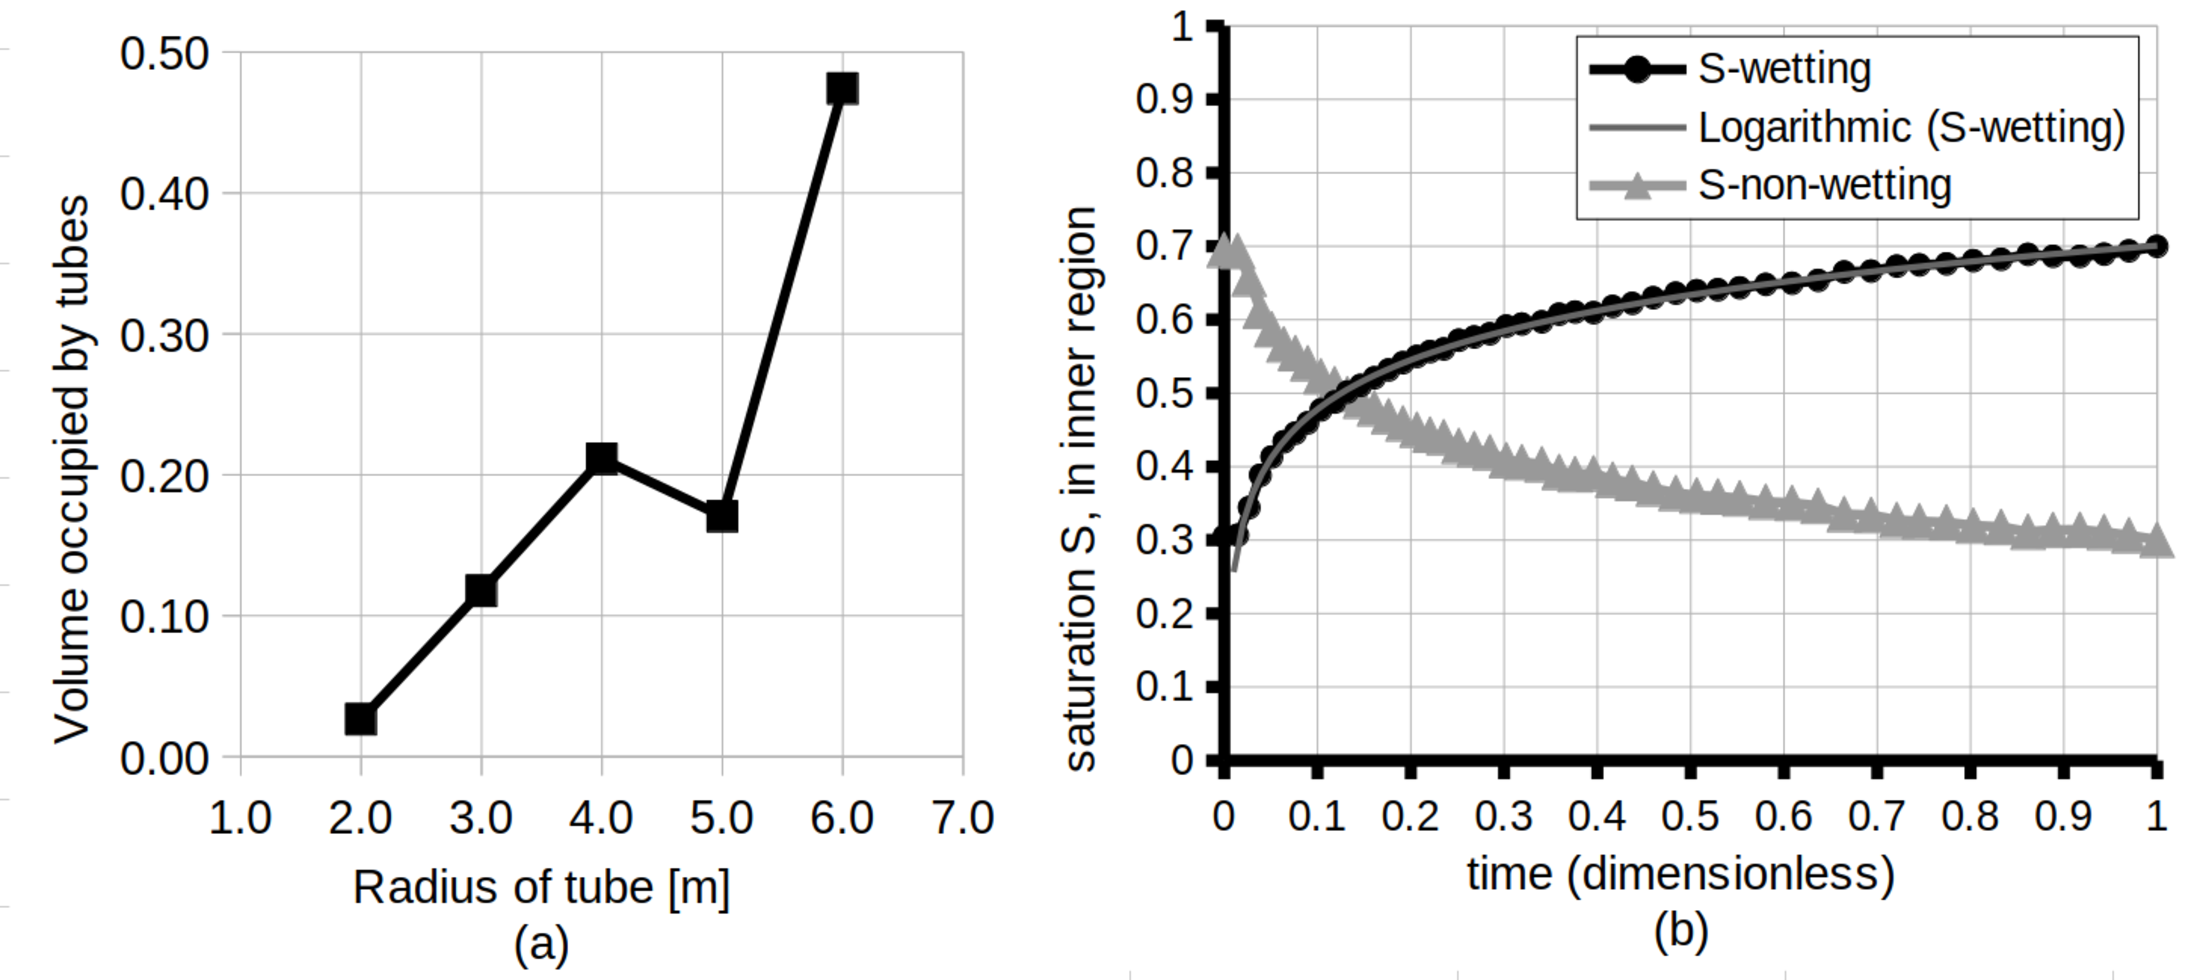
\includegraphics[width=\textwidth]{fig_4_2200x1000}
		\caption{The proportion of volume occupied by tubes of various radii in the inner region (a). The saturation of the wetting fluid in the inner region with respect to time in the inner region (b).}
		\label{fig:4}
	\end{figure}
	
	\begin{figure}
		\centering
		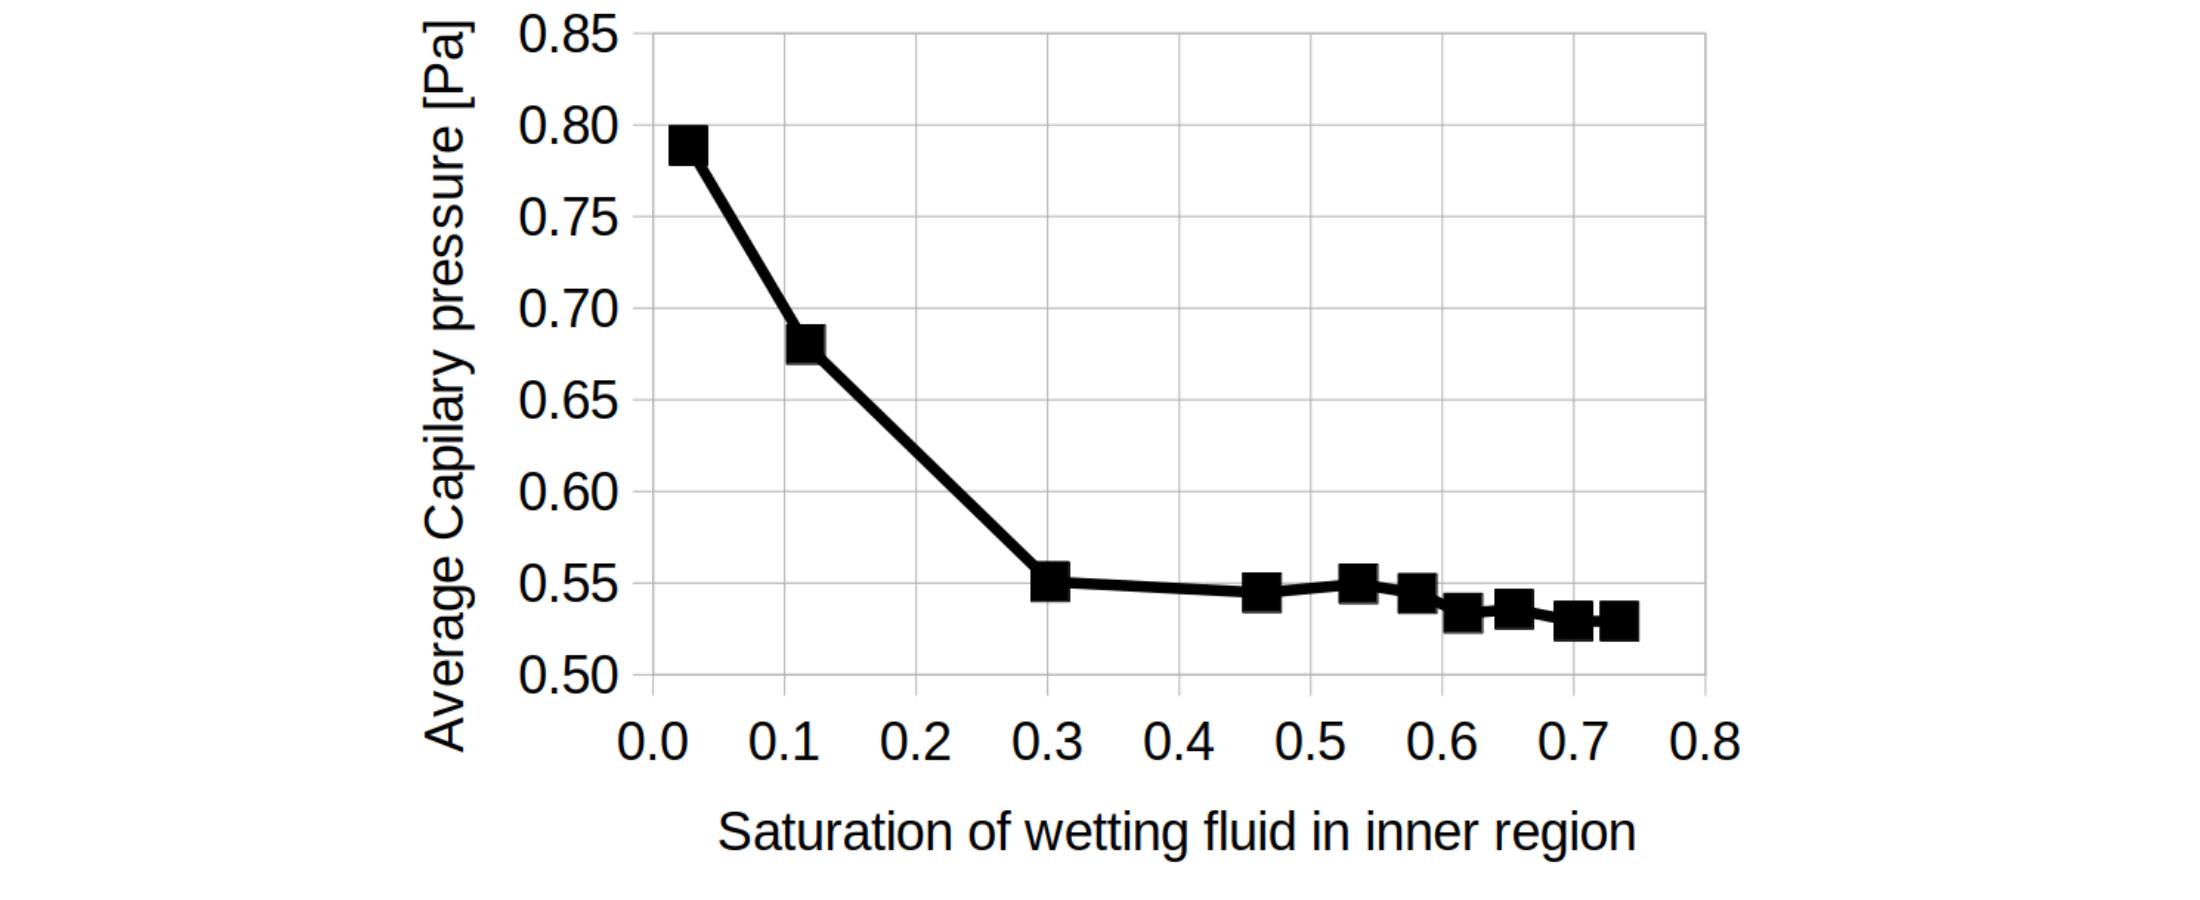
\includegraphics[width=\textwidth]{fig_5_2200x900}
		\caption{Showing the increase of capillary pressure as the saturation of wetting fluid in the inner region decreases.}
		\label{fig:5}
	\end{figure}
	
	
	The algorithm was implemented in C++ 17, compiled using gcc 9.4.0. The computation was performed using processor 11th Gen Intel Core i5-1135G7 @ 2.40GHz operating with Ubuntu 20.04 LTS. Only one core of the processor was used at a time. Each experiment took about 5 minutes to complete.
	
	We studied the accumulation of numerical error accumulation. After solving the set of linear equations we obtain pressures in each node. These pressures are not accurate, because there is numerical error accumulated while solving the set of linear equations. Which results law of conservation of volume very slightly violated in the nodes. The saturation of a particular fluid in whole system must remain the same since we have closed boundaries. However, in the nodes when more than one fluid flows in, the law of conservation of volume is slightly violated due to numerical error, then this results in changes of saturation of a particular fluid in the system. Using data type $float$ in C++ allows 2 to 3 times faster computation, however after $10^4$ steps, we observed that $\Delta S / S \approx 10^{-2}$, which we considered to be significant. But when all the real numbers are processed as $double$ the error is reduced to $\Delta S / S \approx 10^{-4}$.
	
	In figure \ref{fig:4} we see that the wetting fluid invades the inner region and displaces the non-wetting fluid to the outer region. The process happens smoothly over time. The curve can be very well approximated using a logarithmic equation. $S$ tends to an equilibrium value, and hence there is a Kondaurov parameter $\xi$ [REF?] which tends to an equilibrium value. Such plots were similar for all the experiments where the initial saturation of the wetting fluid was varied.
	
	In figure \ref{fig:5} we see that the average final capillary pressure of the inner region increased as we decreased the final saturation of the wetting fluid in the inner region as per \cite{fatt1956network}. Since our network model could maximum consist of $30 \times 30$ rows and columns of tubes, the tubes with thinnest radii could take a very small proportion of the volume of the inner region. In figure \ref{fig:3}b, we see that the darker or non-wetting fluid mostly occupies the intersections of the tubes with the thickest radii while the wetting fluid occupies the thinnest tubes to reduce the free energy of the system. It should be noted that our novel method, even tough just an algorithm to distribute fluids in a node, correctly keeps the wetting fluid in the tubes of thinner radii. Since according to equation \ref{eq:average-capillary-pressure}, tubes with only one type of fluid does not contribute to the total average capillary pressure, then the saturation is very high, the thinnest tubes are most likely to be completely filled, and therefore the tubes with single meniscus are most likely the thickest ones. Since the capillary pressure is inversely proportional to the radius, that is why we see a decrease on average capillary pressure when the saturation of wetting fluid increases in the inner region.
	
	
\section{Conclusion}
	\begin{enumerate}
		\item Our novel method of distributing different fluids in the nodes, such the wetting fluid first goes into the tube with the thinner radius is valid, because the wetting fluid successfully invades the inner region. And, the wetting fluid prefers to remain in the thinner capillaries.
		
		\item We obtained a very smooth plot of $S(t)$. And, the saturation tends to an equilibrium value, according to Kondaurov [REF?].
		
		\item Our custom definition of calculating the average capillary pressure in a network model must be correct because the capillary pressure increases with decrease of saturation of wetting fluid in the inner region.
		
		\item The maximum number of connections a node in our network model can have is 4. It is possible to extend our novel method of distributing fluids at the node to the more connections, which will especially be useful for a 3D network model.
		
		\item The fluid loss in the system is negligible due to the use of Gaussian-elimination for solving the set of linear equations. However the number of nodes is limited to only $10^3$, in order to simulate a porous media with more pores or nodes, it is recommended to use iterative methods.
	\end{enumerate}

\bibliographystyle{plain.bst}
\bibliography{reference}
\end{document}
